%%%%%%%%%%%%%%%%%%%%%%%%%%%%%%%%%%%%%%%%%
% baposter Portrait Poster
% LaTeX Template
% Version 1.0 (15/5/13)
%
% Created by:
% Brian Amberg (baposter@brian-amberg.de)
%
% This template has been downloaded from:
% http://www.LaTeXTemplates.com
%
% License:
% CC BY-NC-SA 3.0 (http://creativecommons.org/licenses/by-nc-sa/3.0/)
%
%%%%%%%%%%%%%%%%%%%%%%%%%%%%%%%%%%%%%%%%%

%----------------------------------------------------------------------------------------
%	PACKAGES AND OTHER DOCUMENT CONFIGURATIONS
%----------------------------------------------------------------------------------------

\documentclass[a0paper,portrait]{baposter}

\usepackage[font=small,labelfont=bf]{caption} % Required for specifying captions to tables and figures
\usepackage{booktabs} % Horizontal rules in tables
\usepackage{relsize} % Used for making text smaller in some places

\usepackage{floatrow}
\newfloatcommand{capbtabbox}{table}[][\FBwidth]
\usepackage{blindtext}
\usepackage{listings}

\usepackage{url}

\graphicspath{{figures/}} % Directory in which figures are stored

\definecolor{bordercol}{RGB}{40,40,40} % Border color of content boxes
\definecolor{headercol1}{RGB}{186,215,230} % Background color for the header in the content boxes (left side)
\definecolor{headercol2}{RGB}{80,80,80} % Background color for the header in the content boxes (right side)
\definecolor{headerfontcol}{RGB}{0,0,0} % Text color for the header text in the content boxes
\definecolor{boxcolor}{RGB}{186,215,230} % Background color for the content in the content boxes

\begin{document}
\lstset{language=SQL}

\background{ % Set the background to an image (background.pdf)
\begin{tikzpicture}[remember picture,overlay]
\draw (current page.north west)+(-2em,2em) node[anchor=north west]
{\includegraphics[height=1.1\textheight]{background}};
\end{tikzpicture}
}

\begin{poster}{
grid=false,
borderColor=bordercol, % Border color of content boxes
headerColorOne=headercol1, % Background color for the header in the content boxes (left side)
headerColorTwo=headercol2, % Background color for the header in the content boxes (right side)
headerFontColor=headerfontcol, % Text color for the header text in the content boxes
boxColorOne=boxcolor, % Background color for the content in the content boxes
headershape=roundedright, % Specify the rounded corner in the content box headers
headerfont=\Large\sf\bf, % Font modifiers for the text in the content box headers
textborder=rectangle,
background=user,
headerborder=open, % Change to closed for a line under the content box headers
boxshade=plain
}
{}
%
%----------------------------------------------------------------------------------------
%	TITLE AND AUTHOR NAME
%----------------------------------------------------------------------------------------
%
{\sf\bf \LARGE{Utilizing Views to Normalize  \texttt{c\_metadataxml} \\ Values in Multi-Axial Metadata Hierarchies}} % Poster title
{\vspace{1em} Hubert Hickman\\ % Author names
{\smaller hhickman@essexmanagement.com}} % Author email addresses
{\includegraphics[scale=0.12]{essex}} % University/lab logo

%----------------------------------------------------------------------------------------
%	INTRODUCTION
%----------------------------------------------------------------------------------------

\headerbox{Introduction}{name=introduction,column=0,row=0}{

With the increasing use of mutli-axial hierarchy metadata in i2b2 systems, the management 
of \texttt{c\_metadataxml} values can become unwieldy.  Since a given \texttt{c\_conceptcd} can 
occur many times in the metadata, steps to normalize these values can be made without changing i2b2 source code.  
}

%----------------------------------------------------------------------------------------
%	MATERIALS AND METHODS
%----------------------------------------------------------------------------------------

\headerbox{Mutli-Axial Hierarchies}{name=methods,column=0,below=introduction}{
Many of the metadata sets used in the i2b2 ontology cell follow a simple parent/child pattern.  That is, for a given node in a i2b2 metadata tree, a child node may have only one parent.  Hence, the leaf node will only occur one time and no \texttt{c\_metadataxml} needs to be defined more than one time.

\vspace{1em} 

However, in a multi-axial hierarchy there can be many paths to reach a particular leaf node.  Hence, each time the leaf node is repeated, the corresponding \texttt{c\_metadataxml} must be replicated in each row of metadata.   

}

%----------------------------------------------------------------------------------------
%	CONCLUSION
%----------------------------------------------------------------------------------------

\headerbox{Conclusion}{name=conclusion,column=0,below=methods}{

The creation of a separate table and a database view for each multi-axial metadata table allows the normalization of the \texttt{c\_metadataxml} field.  This simple solution eliminates the need for maintaining many copies of the \texttt{c\_metadataxml} contents in complex i2b2 ontologies.

\vspace{1em}

An additional normalization could be performed if there exists different data sources at a site with incompatible \texttt{c\_metadataxml} contents for a given \texttt{c\_conceptcd}.  If an additional field for \texttt{c\_sourcesystemcd} is added to the \texttt{metadataxml\_map} table and the view is trivially extended, then the solution will work for many different datasources.
}

%----------------------------------------------------------------------------------------
%	ACKNOWLEDGEMENTS
%----------------------------------------------------------------------------------------

\headerbox{Acknowledgements}{name=acknowledgements,column=0,below=conclusion, above=bottom}{

%\smaller % Reduce the font size in this block
The author gratefully acknowledges the support of Essex Management for allowing me the time to work on i2b2 community oriented work.  I would also like to thank the i2b2 group at the University of Nebraska Medical Center and NYU Langone Medical Center.  Most especially I would like to thank Dr. James R. Campbell, M.D. for getting me involved in i2b2 and metadata development.


\vspace{1em}

The LOINC example pathways are taken from LOINC metadata developed for the GPC CDRN.

} 

%----------------------------------------------------------------------------------------
%	RESULTS 1
%----------------------------------------------------------------------------------------

\headerbox{Sample metadata paths for WBC in LOINC}{name=results1,span=2,column=1,row=0}{ % To reduce this block to 1 column width, remove 'span=2'

 

%------------------------------------------------

    \begin{center}
    %\rule{6.4cm}{3.6cm}
	%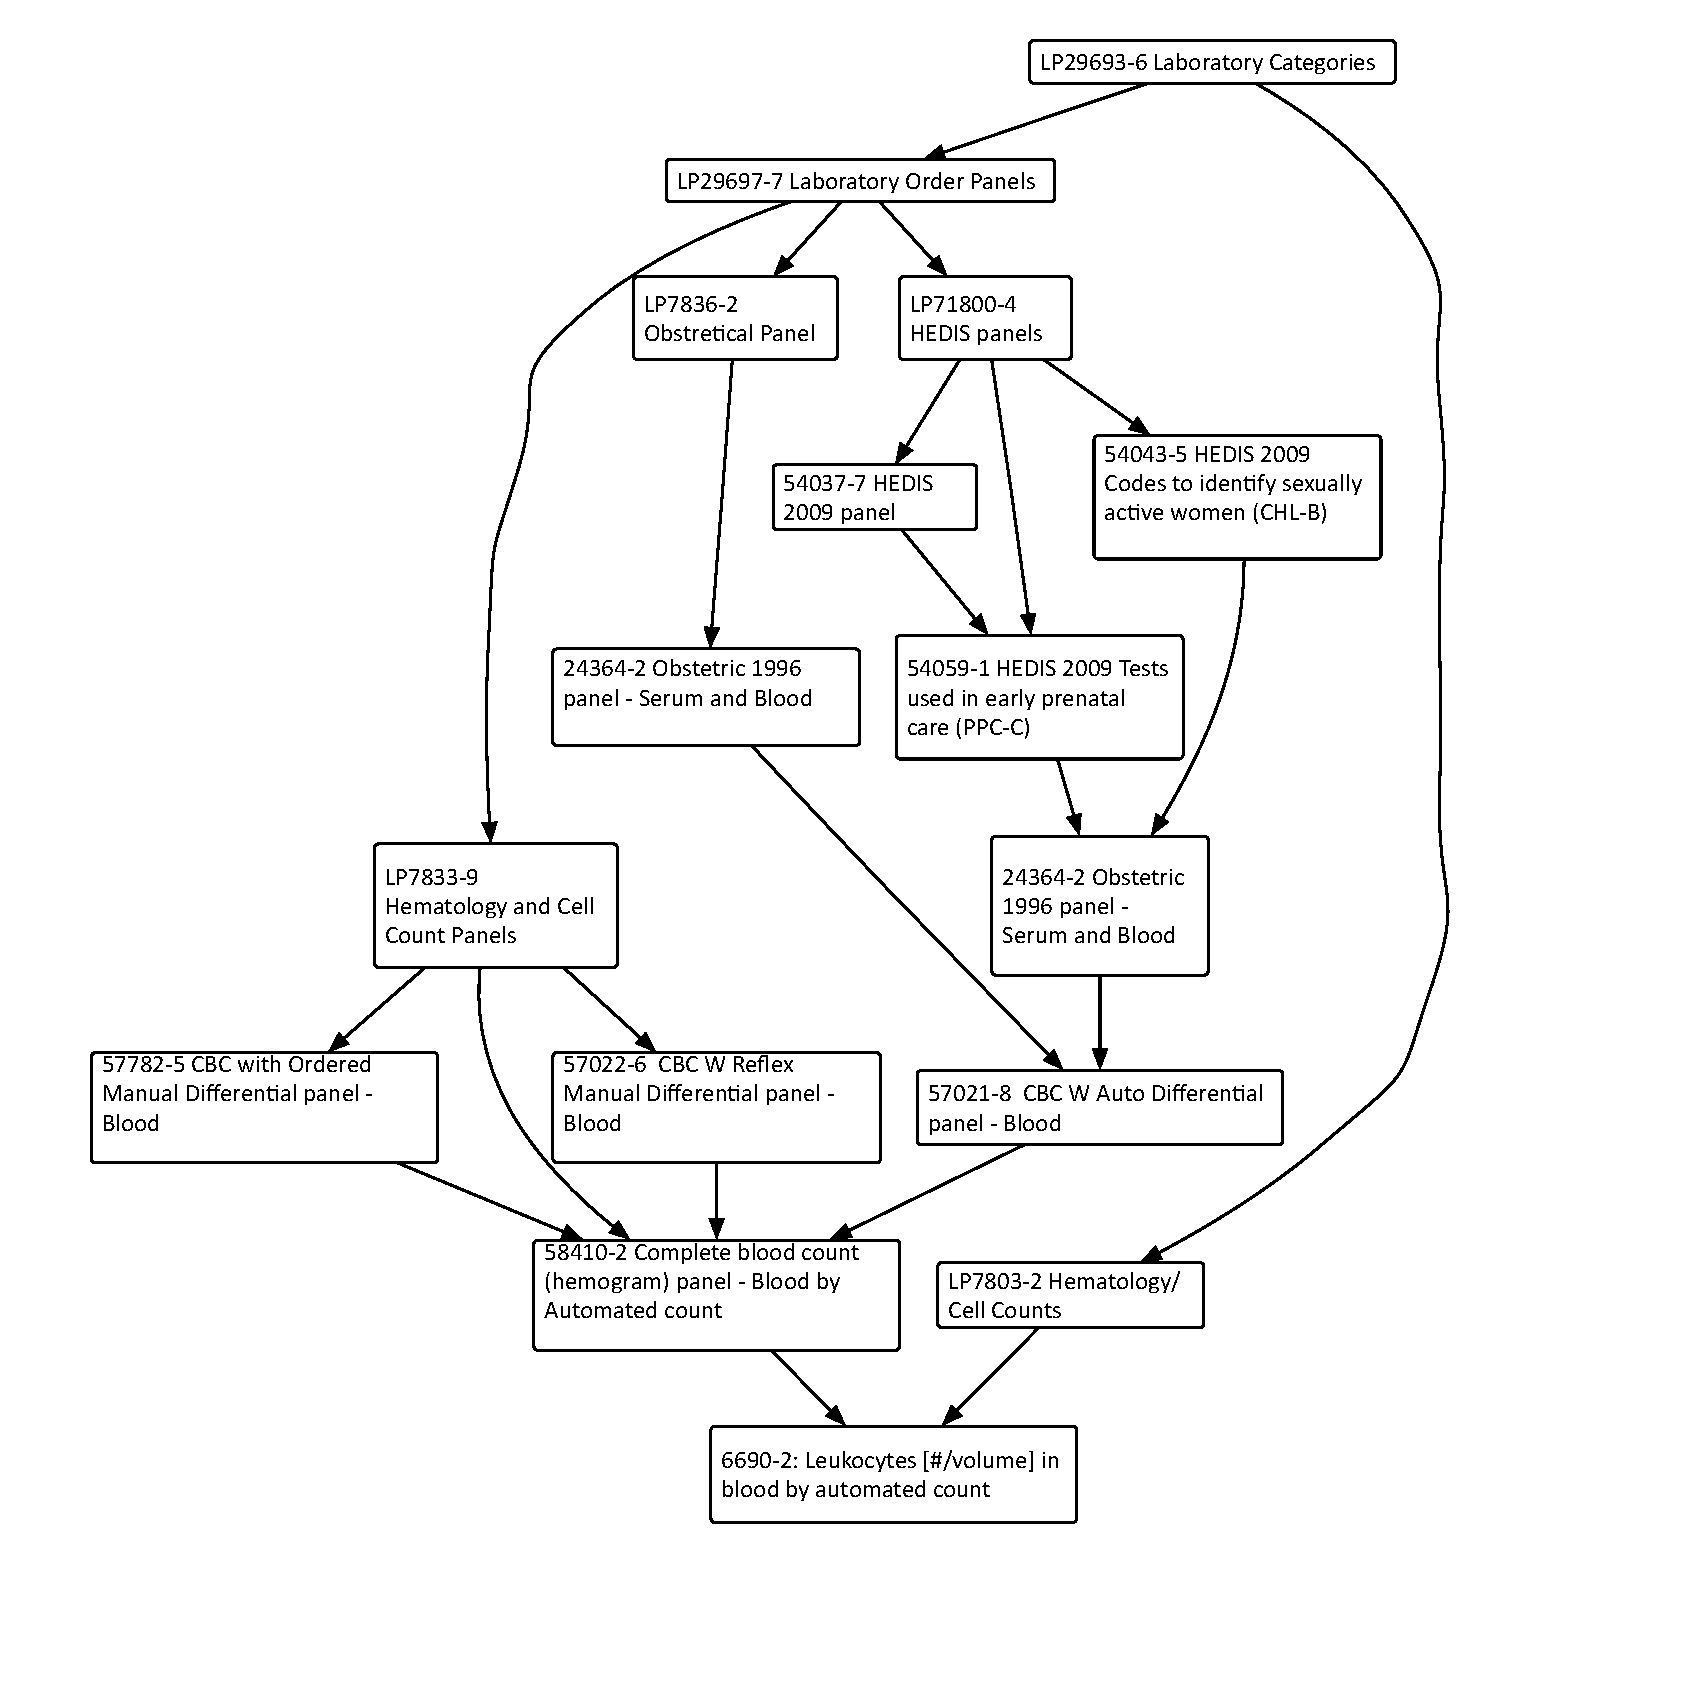
\includegraphics[width=0.59\linewidth, scale=0.5]{diagram1}
		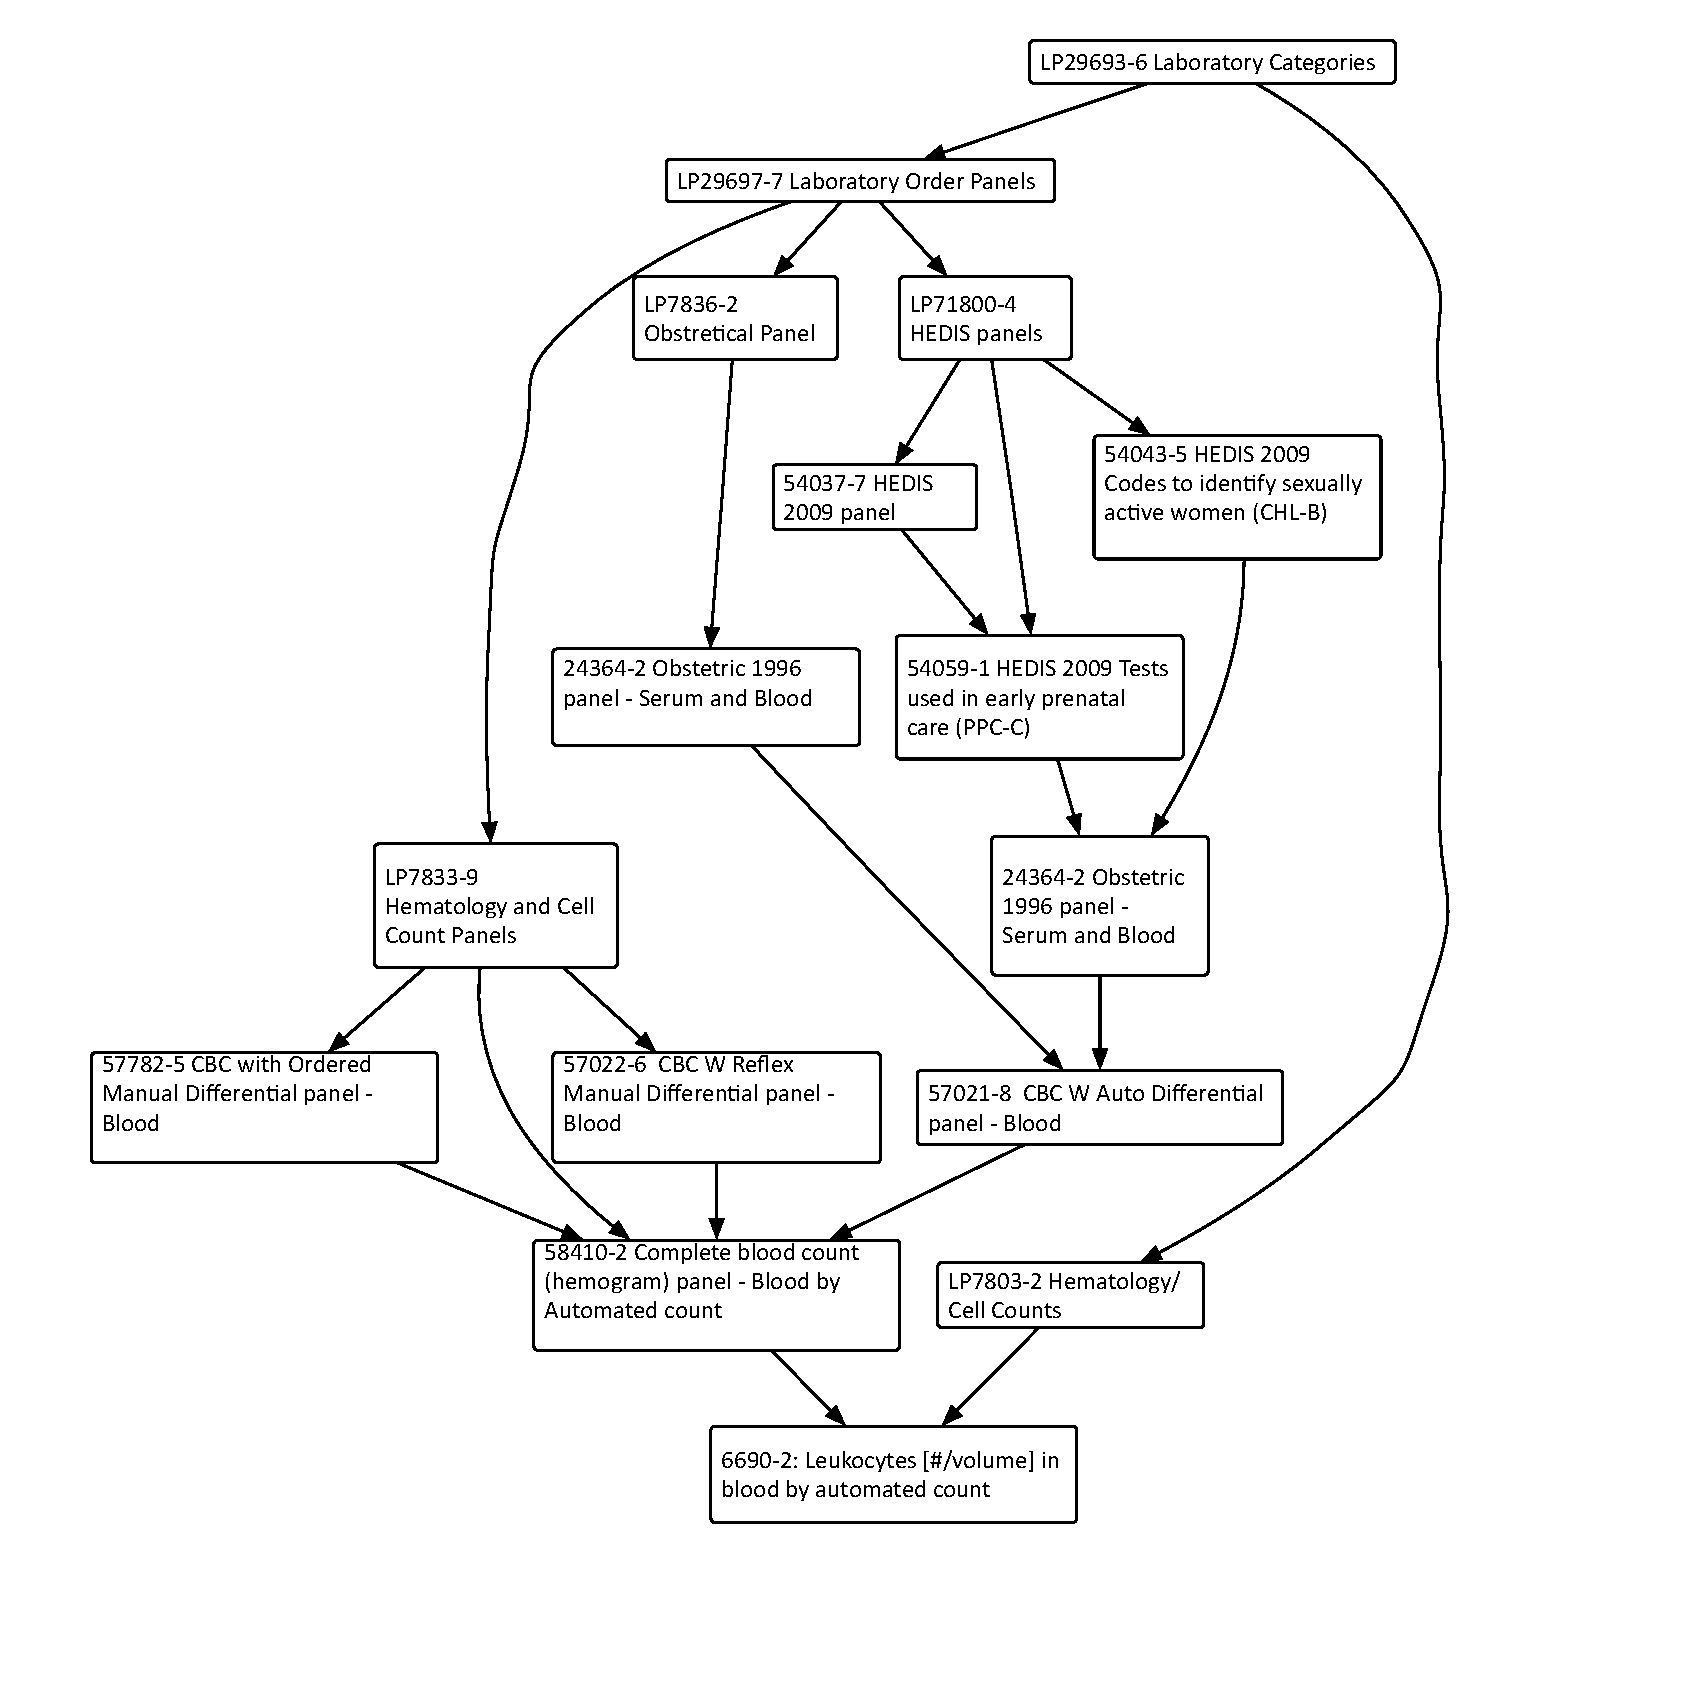
\includegraphics[width=0.5\textwidth]{diagram1}

	\captionof{figure}{Example paths in LOINC}
\end{center}
    The graph shown above shows the different paths by which LOINC 6690-2 can be reached. There exist eight distinct paths from the top level node (Laboratory Categories) the the leaf node. The paths are enumerated in the table below.
\begin{center}
\begin{tabular}{|l|}\hline
      c\_fullname \\ \hline 
      {\footnotesize 
       \textbackslash LP29693-6\textbackslash LP29697-7\textbackslash LP71800-4\textbackslash 54037-7\textbackslash 54059-1\textbackslash 24364-2\textbackslash 57021-8\textbackslash 58410-2\textbackslash 6690-2\textbackslash} \\ \hline 
      {\footnotesize \textbackslash LP29693-6 \textbackslash LP29697-7 \textbackslash LP71800-4 \textbackslash 54059-1\textbackslash 4364-2\textbackslash 57021-8\textbackslash 58410-2\textbackslash 6690-2 \textbackslash }\\ \hline
      {\footnotesize \textbackslash LP29693-6\textbackslash LP29697-7\textbackslash LP71800-4\textbackslash 54043-5\textbackslash 24364-2\textbackslash 57021-8\textbackslash 58410-2\textbackslash 6690-2\textbackslash
      } \\ \hline
      {\footnotesize \textbackslash LP29693-6\textbackslash LP29697-7\textbackslash LP7833-9\textbackslash 57022-6\textbackslash 58410-2\textbackslash 6690-2\textbackslash 
} \\ \hline
{\footnotesize 
\textbackslash LP29693-6\textbackslash LP29697-7\textbackslash LP7833-9 \textbackslash 57782-5\textbackslash 58410-2 \textbackslash 6690-2\textbackslash } \\ \hline 
{\footnotesize 
\textbackslash LP29693-6\textbackslash LP29697-7 \textbackslash LP7833-9\textbackslash 58410-2\textbackslash 6690-2\textbackslash } \\ \hline 
{\footnotesize 
\textbackslash LP29693-6 \textbackslash LP29697-7\textbackslash LP7836-2\textbackslash 24364-2\textbackslash 57021-8\textbackslash 58410-2\textbackslash 6690-2\textbackslash } \\ \hline
{\footnotesize
\textbackslash LP29693-6\textbackslash LP7803-2\textbackslash 6690-2 \textbackslash } \\ \hline 

      \end{tabular}
      \captionof{table}{Sample Metadata Paths for LOINC 6690-2}
      \end{center}

}

%----------------------------------------------------------------------------------------
%	RESULTS 2
%----------------------------------------------------------------------------------------

\headerbox{Adding Views to the Ontology Schema}{name=results2,span=2,column=1,below=results1,above=bottom}{ % To reduce this block to 1 column width, remove 'span=2'

The goal is to create a metadata view that encompasses the normalization of the \texttt{c\_metadata} field. To accomplish this goal, we add a new table that contains the \texttt{c\_metadataxml} field and the \texttt{c\_basecode} field.

\vspace{1em}

The view definition as shown above is very simple.  One needs to use care when performing fact counting procedures that update the metadata tables and use the physical metadata table, and the not the view.

\begin{center}
\lstinputlisting{newsql.txt} 
\end{center}
%------------------------------------------------

%\begin{center}
%\includegraphics[width=0.49\linewidth]{placeholder}
%\includegraphics[width=0.49\linewidth]{placeholder}
%\captionof{figure}{Figure caption 1 (left); Figure caption 2 (right)}
%\end{center}

%------------------------------------------------

With the new table, each \texttt{c\_basecode} value only occurs one time.  In the \texttt{table\_access} table, the view name is substituted for the the original table.
}

%----------------------------------------------------------------------------------------

\end{poster}



\end{document}